\documentclass[twoside]{article}

% Packages required by doxygen
\usepackage{fixltx2e}
\usepackage{calc}
\usepackage{doxygen}
\usepackage[export]{adjustbox} % also loads graphicx
\usepackage{graphicx}
\usepackage[utf8]{inputenc}
\usepackage{makeidx}
\usepackage{multicol}
\usepackage{multirow}
\PassOptionsToPackage{warn}{textcomp}
\usepackage{textcomp}
\usepackage[nointegrals]{wasysym}
\usepackage[table]{xcolor}

% Font selection
\usepackage[T1]{fontenc}
\usepackage[scaled=.90]{helvet}
\usepackage{courier}
\usepackage{amssymb}
\usepackage{sectsty}
\renewcommand{\familydefault}{\sfdefault}
\allsectionsfont{%
  \fontseries{bc}\selectfont%
  \color{darkgray}%
}
\renewcommand{\DoxyLabelFont}{%
  \fontseries{bc}\selectfont%
  \color{darkgray}%
}
\newcommand{\+}{\discretionary{\mbox{\scriptsize$\hookleftarrow$}}{}{}}

% Page & text layout
\usepackage{geometry}
\geometry{%
  a4paper,%
  top=2.5cm,%
  bottom=2.5cm,%
  left=2.5cm,%
  right=2.5cm%
}
\tolerance=750
\hfuzz=15pt
\hbadness=750
\setlength{\emergencystretch}{15pt}
\setlength{\parindent}{0cm}
\setlength{\parskip}{3ex plus 2ex minus 2ex}
\makeatletter
\renewcommand{\paragraph}{%
  \@startsection{paragraph}{4}{0ex}{-1.0ex}{1.0ex}{%
    \normalfont\normalsize\bfseries\SS@parafont%
  }%
}
\renewcommand{\subparagraph}{%
  \@startsection{subparagraph}{5}{0ex}{-1.0ex}{1.0ex}{%
    \normalfont\normalsize\bfseries\SS@subparafont%
  }%
}
\makeatother

% Headers & footers
\usepackage{fancyhdr}
\pagestyle{fancyplain}
\fancyhead[LE]{\fancyplain{}{\bfseries\thepage}}
\fancyhead[CE]{\fancyplain{}{}}
\fancyhead[RE]{\fancyplain{}{\bfseries\leftmark}}
\fancyhead[LO]{\fancyplain{}{\bfseries\rightmark}}
\fancyhead[CO]{\fancyplain{}{}}
\fancyhead[RO]{\fancyplain{}{\bfseries\thepage}}
\fancyfoot[LE]{\fancyplain{}{}}
\fancyfoot[CE]{\fancyplain{}{}}
\fancyfoot[RE]{\fancyplain{}{\bfseries\scriptsize Generated by Doxygen }}
\fancyfoot[LO]{\fancyplain{}{\bfseries\scriptsize Generated by Doxygen }}
\fancyfoot[CO]{\fancyplain{}{}}
\fancyfoot[RO]{\fancyplain{}{}}
\renewcommand{\footrulewidth}{0.4pt}
\renewcommand{\sectionmark}[1]{%
  \markright{\thesection\ #1}%
}

% Indices & bibliography
\usepackage{natbib}
\usepackage[titles]{tocloft}
\setcounter{tocdepth}{3}
\setcounter{secnumdepth}{5}
\makeindex

% Hyperlinks (required, but should be loaded last)
\usepackage{ifpdf}
\ifpdf
  \usepackage[pdftex,pagebackref=true]{hyperref}
\else
  \usepackage[ps2pdf,pagebackref=true]{hyperref}
\fi
\hypersetup{%
  colorlinks=true,%
  linkcolor=blue,%
  citecolor=blue,%
  unicode%
}

% Custom commands
\newcommand{\clearemptydoublepage}{%
  \newpage{\pagestyle{empty}\cleardoublepage}%
}

\usepackage{caption}
\captionsetup{labelsep=space,justification=centering,font={bf},singlelinecheck=off,skip=4pt,position=top}

%===== C O N T E N T S =====

\begin{document}

% Titlepage & ToC
\hypersetup{pageanchor=false,
             bookmarksnumbered=true,
             pdfencoding=unicode
            }
\pagenumbering{roman}
\begin{titlepage}
\vspace*{7cm}
\begin{center}%
{\Large P\+A09-\/\+Heap }\\
\vspace*{1cm}
{\large Generated by Doxygen 1.8.11}\\
\end{center}
\end{titlepage}
\tableofcontents
\pagenumbering{arabic}
\hypersetup{pageanchor=true}

%--- Begin generated contents ---
\section{Main Page}
\label{index}\hypertarget{index}{}This project contains the following items -\/create an implementation of the Weighted Graph A\+DT usin ga vertex list and an adjacency matrix. -\/\+Develop a routine that finds the shorted path between each pair of vertices in a graph. -\/add vertex coloring and implement a function that checks whether a graph has a proper coloring. -\/investiate the four color theorem by generating a graph for which no proper coloring can be creating using less than five colors. 
\section{Hierarchical Index}
\subsection{Class Hierarchy}
This inheritance list is sorted roughly, but not completely, alphabetically\+:\begin{DoxyCompactList}
\item \contentsline{section}{Greater$<$ Key\+Type $>$}{\pageref{class_greater}}{}
\item \contentsline{section}{Heap$<$ Data\+Type, Key\+Type, Comparator $>$}{\pageref{class_heap}}{}
\item \contentsline{section}{Heap$<$ Data\+Type $>$}{\pageref{class_heap}}{}
\begin{DoxyCompactList}
\item \contentsline{section}{Priority\+Queue$<$ Data\+Type, Key\+Type, Comparator $>$}{\pageref{class_priority_queue}}{}
\end{DoxyCompactList}
\item \contentsline{section}{Less$<$ Key\+Type $>$}{\pageref{class_less}}{}
\item \contentsline{section}{Less$<$ int $>$}{\pageref{class_less}}{}
\item \contentsline{section}{Task\+Data}{\pageref{struct_task_data}}{}
\item \contentsline{section}{Test\+Data}{\pageref{class_test_data}}{}
\item \contentsline{section}{Test\+Data\+Item$<$ Key\+Type $>$}{\pageref{class_test_data_item}}{}
\end{DoxyCompactList}

\section{Class Index}
\subsection{Class List}
Here are the classes, structs, unions and interfaces with brief descriptions\+:\begin{DoxyCompactList}
\item\contentsline{section}{\hyperlink{classbinary_search}{binary\+Search} }{\pageref{classbinary_search}}{}
\item\contentsline{section}{\hyperlink{classlinear_search}{linear\+Search} }{\pageref{classlinear_search}}{}
\item\contentsline{section}{\hyperlink{class_search}{Search} }{\pageref{class_search}}{}
\item\contentsline{section}{\hyperlink{class_s_t_l_search}{S\+T\+L\+Search} }{\pageref{class_s_t_l_search}}{}
\item\contentsline{section}{\hyperlink{class_test_vector}{Test\+Vector} }{\pageref{class_test_vector}}{}
\item\contentsline{section}{\hyperlink{class_timer}{Timer} }{\pageref{class_timer}}{}
\end{DoxyCompactList}

\section{File Index}
\subsection{File List}
Here is a list of all files with brief descriptions\+:\begin{DoxyCompactList}
\item\contentsline{section}{\hyperlink{okay_8cpp}{okay.\+cpp} }{\pageref{okay_8cpp}}{}
\item\contentsline{section}{\hyperlink{_rush_hour_8cpp}{Rush\+Hour.\+cpp} }{\pageref{_rush_hour_8cpp}}{}
\end{DoxyCompactList}

\section{Class Documentation}
\hypertarget{class_greater}{}\subsection{Greater$<$ Key\+Type $>$ Class Template Reference}
\label{class_greater}\index{Greater$<$ Key\+Type $>$@{Greater$<$ Key\+Type $>$}}
\subsubsection*{Public Member Functions}
\begin{DoxyCompactItemize}
\item 
bool {\bfseries operator()} (const Key\+Type \&a, const Key\+Type \&b) const \hypertarget{class_greater_a79d9cb7121723ee9d65b11cb2fce0379}{}\label{class_greater_a79d9cb7121723ee9d65b11cb2fce0379}

\end{DoxyCompactItemize}


The documentation for this class was generated from the following file\+:\begin{DoxyCompactItemize}
\item 
test11.\+cpp\end{DoxyCompactItemize}

\hypertarget{class_heap}{}\subsection{Heap$<$ Data\+Type, Key\+Type, Comparator $>$ Class Template Reference}
\label{class_heap}\index{Heap$<$ Data\+Type, Key\+Type, Comparator $>$@{Heap$<$ Data\+Type, Key\+Type, Comparator $>$}}
\subsubsection*{Public Member Functions}
\begin{DoxyCompactItemize}
\item 
\hyperlink{class_heap_ae17e34e3c86d88263a8fdf80b9ba78fc}{Heap} (int max\+Number=D\+E\+F\+A\+U\+L\+T\+\_\+\+M\+A\+X\+\_\+\+H\+E\+A\+P\+\_\+\+S\+I\+ZE)
\item 
\hyperlink{class_heap_a97e3b462be1c6af31d7519546bba8907}{Heap} (const \hyperlink{class_heap}{Heap} \&other)
\item 
\hyperlink{class_heap}{Heap} \& \hyperlink{class_heap_a5ed119341c39bcea1437321d4247dd40}{operator=} (const \hyperlink{class_heap}{Heap} \&other)
\item 
\hyperlink{class_heap_a555ade7891007de959bef0ee53e28767}{$\sim$\+Heap} ()
\item 
void \hyperlink{class_heap_aa68cf80454ab1b246fa723612805a91e}{insert} (const Data\+Type \&new\+Data\+Item)  throw ( logic\+\_\+error )
\item 
Data\+Type \hyperlink{class_heap_a4a18bfdacd897c45fc3da13f22b8930d}{remove} ()  throw ( logic\+\_\+error )
\item 
void \hyperlink{class_heap_a19a78c8eae2cf7c8253e34e54d86ed73}{clear} ()
\item 
bool \hyperlink{class_heap_ab8fa26d416ac0e27dfcbf18c54f8f73f}{is\+Empty} () const 
\item 
bool \hyperlink{class_heap_ac9111b884c74a376240e0155a788756e}{is\+Full} () const 
\item 
void \hyperlink{class_heap_a3ae1e1f27a145749c8b9f2da777cb8bc}{show\+Structure} () const 
\item 
void \hyperlink{class_heap_a4bdb1772ea92899de245d6cbd217d085}{write\+Levels} () const 
\end{DoxyCompactItemize}
\subsubsection*{Static Public Attributes}
\begin{DoxyCompactItemize}
\item 
static const int {\bfseries D\+E\+F\+A\+U\+L\+T\+\_\+\+M\+A\+X\+\_\+\+H\+E\+A\+P\+\_\+\+S\+I\+ZE} = 10\hypertarget{class_heap_a967c19732a20a72e8e824402ad6763c8}{}\label{class_heap_a967c19732a20a72e8e824402ad6763c8}

\end{DoxyCompactItemize}
\subsubsection*{Private Member Functions}
\begin{DoxyCompactItemize}
\item 
void \hyperlink{class_heap_a49a54dd4782e6c68f14a5df3ba4da7af}{show\+Subtree} (int index, int level) const 
\item 
int \hyperlink{class_heap_a85f4db6e6ffa391ad5bebfd26a65fe57}{Parent} (int child)
\item 
int \hyperlink{class_heap_a0b6b9d7ed6c60593064098153d488ae4}{Left\+Child} (int parent)
\item 
int \hyperlink{class_heap_a16a5a9019f1f175f285a0457361cfcf0}{Right\+Child} (int parent)
\item 
void \hyperlink{class_heap_a57a70833393f66b6504efc02676a1ac5}{swap} (int index1, int index2)
\end{DoxyCompactItemize}
\subsubsection*{Private Attributes}
\begin{DoxyCompactItemize}
\item 
int {\bfseries max\+Size}\hypertarget{class_heap_a7f8e5c3cc64b8799b4e75b5a0f675e69}{}\label{class_heap_a7f8e5c3cc64b8799b4e75b5a0f675e69}

\item 
int {\bfseries size}\hypertarget{class_heap_a0964c2d309605bee2f6f1a9cee9ab89a}{}\label{class_heap_a0964c2d309605bee2f6f1a9cee9ab89a}

\item 
Data\+Type $\ast$ {\bfseries data\+Items}\hypertarget{class_heap_ace779ec73409a031eda4a7c1b898eb56}{}\label{class_heap_ace779ec73409a031eda4a7c1b898eb56}

\item 
Comparator {\bfseries comparator}\hypertarget{class_heap_adc20ebd4d97dff37f19ced91ccdc4560}{}\label{class_heap_adc20ebd4d97dff37f19ced91ccdc4560}

\end{DoxyCompactItemize}


\subsubsection{Constructor \& Destructor Documentation}
\index{Heap@{Heap}!Heap@{Heap}}
\index{Heap@{Heap}!Heap@{Heap}}
\paragraph[{\texorpdfstring{Heap(int max\+Number=\+D\+E\+F\+A\+U\+L\+T\+\_\+\+M\+A\+X\+\_\+\+H\+E\+A\+P\+\_\+\+S\+I\+Z\+E)}{Heap(int maxNumber=DEFAULT_MAX_HEAP_SIZE)}}]{\setlength{\rightskip}{0pt plus 5cm}template$<$typename Data\+Type , typename Key\+Type , typename Comparator $>$ {\bf Heap}$<$ Data\+Type, Key\+Type, Comparator $>$\+::{\bf Heap} (
\begin{DoxyParamCaption}
\item[{int}]{max\+Number = {\ttfamily DEFAULT\+\_\+MAX\+\_\+HEAP\+\_\+SIZE}}
\end{DoxyParamCaption}
)}\hypertarget{class_heap_ae17e34e3c86d88263a8fdf80b9ba78fc}{}\label{class_heap_ae17e34e3c86d88263a8fdf80b9ba78fc}
This function is the param constructor for the \hyperlink{class_heap}{Heap} class.

This function will set the max\+Size equal to the parameter max\+Number passed in. This function will set the size to 0 since we are not putting in any data yet. This function will dynamically allocate memory for the array of Data\+Type with max\+Size.


\begin{DoxyParams}{Parameters}
{\em int} & max\+Number, which is the largest possible size for the heap. \\
\hline
\end{DoxyParams}
\begin{DoxyReturn}{Returns}
This function does not return anything.
\end{DoxyReturn}
\begin{DoxyPrecond}{Precondition}
none 
\end{DoxyPrecond}
\begin{DoxyPostcond}{Postcondition}
The heap is empty and was just created. 
\end{DoxyPostcond}
\index{Heap@{Heap}!Heap@{Heap}}
\index{Heap@{Heap}!Heap@{Heap}}
\paragraph[{\texorpdfstring{Heap(const Heap \&other)}{Heap(const Heap &other)}}]{\setlength{\rightskip}{0pt plus 5cm}template$<$typename Data\+Type , typename Key\+Type , typename Comparator $>$ {\bf Heap}$<$ Data\+Type, Key\+Type, Comparator $>$\+::{\bf Heap} (
\begin{DoxyParamCaption}
\item[{const {\bf Heap}$<$ Data\+Type, Key\+Type, Comparator $>$ \&}]{other}
\end{DoxyParamCaption}
)}\hypertarget{class_heap_a97e3b462be1c6af31d7519546bba8907}{}\label{class_heap_a97e3b462be1c6af31d7519546bba8907}
This function is the copy constructor for the \hyperlink{class_heap}{Heap} class.

This function will set the max\+Size equal to the other heap\textquotesingle{}s max\+Size. This function will set the size equal to the other heap\textquotesingle{}s size. This function will dynamically allocate memory for the array of Data\+Type with max\+Size. This function will iterate a for loop for the max\+Size until it copies the data of the other heap\textquotesingle{}s data\+Items array into this heap\textquotesingle{}s data\+Items array.


\begin{DoxyParams}{Parameters}
{\em const} & \hyperlink{class_heap}{Heap}\& other which is the other object to be copied to make this object \\
\hline
\end{DoxyParams}
\begin{DoxyReturn}{Returns}
This function does not return anything.
\end{DoxyReturn}
\begin{DoxyPrecond}{Precondition}
none 
\end{DoxyPrecond}
\begin{DoxyPostcond}{Postcondition}
This heap is an exact copy of the other object that was passed in. 
\end{DoxyPostcond}
\index{Heap@{Heap}!````~Heap@{$\sim$\+Heap}}
\index{````~Heap@{$\sim$\+Heap}!Heap@{Heap}}
\paragraph[{\texorpdfstring{$\sim$\+Heap()}{~Heap()}}]{\setlength{\rightskip}{0pt plus 5cm}template$<$typename Data\+Type , typename Key\+Type , typename Comparator $>$ {\bf Heap}$<$ Data\+Type, Key\+Type, Comparator $>$\+::$\sim${\bf Heap} (
\begin{DoxyParamCaption}
{}
\end{DoxyParamCaption}
)}\hypertarget{class_heap_a555ade7891007de959bef0ee53e28767}{}\label{class_heap_a555ade7891007de959bef0ee53e28767}
This function is the destructor for the \hyperlink{class_heap}{Heap} class.

This function will call the clear function to clear the data\+Items array. This function will call the delete operator on data\+Items. This function will set data\+Items to N\+U\+LL.


\begin{DoxyParams}{Parameters}
{\em none} & \\
\hline
\end{DoxyParams}
\begin{DoxyReturn}{Returns}
none
\end{DoxyReturn}
\begin{DoxyPrecond}{Precondition}
none 
\end{DoxyPrecond}
\begin{DoxyPostcond}{Postcondition}
data\+Items will be cleared and deleted and set to N\+U\+LL. 
\end{DoxyPostcond}


\subsubsection{Member Function Documentation}
\index{Heap@{Heap}!clear@{clear}}
\index{clear@{clear}!Heap@{Heap}}
\paragraph[{\texorpdfstring{clear()}{clear()}}]{\setlength{\rightskip}{0pt plus 5cm}template$<$typename Data\+Type , typename Key\+Type , typename Comparator $>$ void {\bf Heap}$<$ Data\+Type, Key\+Type, Comparator $>$\+::clear (
\begin{DoxyParamCaption}
{}
\end{DoxyParamCaption}
)}\hypertarget{class_heap_a19a78c8eae2cf7c8253e34e54d86ed73}{}\label{class_heap_a19a78c8eae2cf7c8253e34e54d86ed73}
This function is the clear function for the \hyperlink{class_heap}{Heap} class.

This function calls the remove function while the is\+Empty function is called. The function keeps calling the remove functio until the heap is empty.


\begin{DoxyParams}{Parameters}
{\em none} & \\
\hline
\end{DoxyParams}
\begin{DoxyReturn}{Returns}
This function does not return anything
\end{DoxyReturn}
\begin{DoxyPrecond}{Precondition}
none 
\end{DoxyPrecond}
\begin{DoxyPostcond}{Postcondition}
This function will clear the data\+Items array in the heap class and make sure that the size is 0. 
\end{DoxyPostcond}
\index{Heap@{Heap}!insert@{insert}}
\index{insert@{insert}!Heap@{Heap}}
\paragraph[{\texorpdfstring{insert(const Data\+Type \&new\+Data\+Item)}{insert(const DataType &newDataItem)}}]{\setlength{\rightskip}{0pt plus 5cm}template$<$typename Data\+Type, typename Key\+Type , typename Comparator $>$ void {\bf Heap}$<$ Data\+Type, Key\+Type, Comparator $>$\+::insert (
\begin{DoxyParamCaption}
\item[{const Data\+Type \&}]{new\+Data\+Item}
\end{DoxyParamCaption}
) throw  logic\+\_\+error) }\hypertarget{class_heap_aa68cf80454ab1b246fa723612805a91e}{}\label{class_heap_aa68cf80454ab1b246fa723612805a91e}
This function is the insert function for the \hyperlink{class_heap}{Heap} class.

The function first checks to see if the heap is full, if it is, the function throws a logic error. Otherwise the function creates an index called child that is equal to the size of the array. The Function then inserts the data\+Item passed into the child index of the array. The Function then incremenets the size. The Function runs in a while loop where child is greater than 0 and by calling the comparator function which checks to see if the value of the new\+Data\+Item is smaller than the parent of the newly inserted data\+Item. If that statement is true, the while loop runs and calls swap with the Parent of the child and child as the parameters. The function then sets child equal to the Parent of the current index since they were swapped. The while loop runs until one of the statements is false, which will finish rearranging the heap.


\begin{DoxyParams}{Parameters}
{\em const} & Data\+Type \&new\+Data\+Item which is the new item to be inserted into the heap \\
\hline
\end{DoxyParams}
\begin{DoxyReturn}{Returns}
This function does not return anything
\end{DoxyReturn}
\begin{DoxyPrecond}{Precondition}
A heap so that items may be inserted into. 
\end{DoxyPrecond}
\begin{DoxyPostcond}{Postcondition}
This function will insert the new\+Data\+Item and rearrange the heap accordingly. 
\end{DoxyPostcond}
\index{Heap@{Heap}!is\+Empty@{is\+Empty}}
\index{is\+Empty@{is\+Empty}!Heap@{Heap}}
\paragraph[{\texorpdfstring{is\+Empty() const }{isEmpty() const }}]{\setlength{\rightskip}{0pt plus 5cm}template$<$typename Data\+Type , typename Key\+Type , typename Comparator $>$ bool {\bf Heap}$<$ Data\+Type, Key\+Type, Comparator $>$\+::is\+Empty (
\begin{DoxyParamCaption}
{}
\end{DoxyParamCaption}
) const}\hypertarget{class_heap_ab8fa26d416ac0e27dfcbf18c54f8f73f}{}\label{class_heap_ab8fa26d416ac0e27dfcbf18c54f8f73f}
This function is the is\+Empty function for the \hyperlink{class_heap}{Heap} class.

This function checks to see if size is equal to 0. If it is, the function returns true. Otherwise the function returns false.


\begin{DoxyParams}{Parameters}
{\em none} & \\
\hline
\end{DoxyParams}
\begin{DoxyReturn}{Returns}
This function returns if the heap is empty or not.
\end{DoxyReturn}
\begin{DoxyPrecond}{Precondition}
none 
\end{DoxyPrecond}
\begin{DoxyPostcond}{Postcondition}
This function will return if the heap is empty or not. 
\end{DoxyPostcond}
\index{Heap@{Heap}!is\+Full@{is\+Full}}
\index{is\+Full@{is\+Full}!Heap@{Heap}}
\paragraph[{\texorpdfstring{is\+Full() const }{isFull() const }}]{\setlength{\rightskip}{0pt plus 5cm}template$<$typename Data\+Type , typename Key\+Type , typename Comparator $>$ bool {\bf Heap}$<$ Data\+Type, Key\+Type, Comparator $>$\+::is\+Full (
\begin{DoxyParamCaption}
{}
\end{DoxyParamCaption}
) const}\hypertarget{class_heap_ac9111b884c74a376240e0155a788756e}{}\label{class_heap_ac9111b884c74a376240e0155a788756e}
This function is the is\+Full function for the \hyperlink{class_heap}{Heap} class.

This function checks to see if size is equal to the max\+Size. If it is, the function returns true. Otherwise the function returns false.


\begin{DoxyParams}{Parameters}
{\em none} & \\
\hline
\end{DoxyParams}
\begin{DoxyReturn}{Returns}
This function returns if the heap is full or not.
\end{DoxyReturn}
\begin{DoxyPrecond}{Precondition}
none 
\end{DoxyPrecond}
\begin{DoxyPostcond}{Postcondition}
This function will return if the heap is fullor not. 
\end{DoxyPostcond}
\index{Heap@{Heap}!Left\+Child@{Left\+Child}}
\index{Left\+Child@{Left\+Child}!Heap@{Heap}}
\paragraph[{\texorpdfstring{Left\+Child(int parent)}{LeftChild(int parent)}}]{\setlength{\rightskip}{0pt plus 5cm}template$<$typename Data\+Type , typename Key\+Type , typename Comparator $>$ int {\bf Heap}$<$ Data\+Type, Key\+Type, Comparator $>$\+::Left\+Child (
\begin{DoxyParamCaption}
\item[{int}]{parent}
\end{DoxyParamCaption}
)\hspace{0.3cm}{\ttfamily [private]}}\hypertarget{class_heap_a0b6b9d7ed6c60593064098153d488ae4}{}\label{class_heap_a0b6b9d7ed6c60593064098153d488ae4}
This function is the Left\+Child function for the \hyperlink{class_heap}{Heap} class.

This function will take the parent and multiply the parent by 2 and add 1. This algorithm can be found in the C++ datastructure course textbook.


\begin{DoxyParams}{Parameters}
{\em int} & parent which is used to find the left child of the parent \\
\hline
\end{DoxyParams}
\begin{DoxyReturn}{Returns}
This function will return the index of the left child of the parent
\end{DoxyReturn}
\begin{DoxyPrecond}{Precondition}
none 
\end{DoxyPrecond}
\begin{DoxyPostcond}{Postcondition}
This function will return the left child index from the parent index that was passed in. 
\end{DoxyPostcond}
\index{Heap@{Heap}!operator=@{operator=}}
\index{operator=@{operator=}!Heap@{Heap}}
\paragraph[{\texorpdfstring{operator=(const Heap \&other)}{operator=(const Heap &other)}}]{\setlength{\rightskip}{0pt plus 5cm}template$<$typename Data\+Type , typename Key\+Type , typename Comparator $>$ {\bf Heap}$<$ Data\+Type, Key\+Type, Comparator $>$ \& {\bf Heap}$<$ Data\+Type, Key\+Type, Comparator $>$\+::operator= (
\begin{DoxyParamCaption}
\item[{const {\bf Heap}$<$ Data\+Type, Key\+Type, Comparator $>$ \&}]{other}
\end{DoxyParamCaption}
)}\hypertarget{class_heap_a5ed119341c39bcea1437321d4247dd40}{}\label{class_heap_a5ed119341c39bcea1437321d4247dd40}
This function is the overloaded assignment operator for the \hyperlink{class_heap}{Heap} class.

This function will first check to see that the other object is not the same as this object. This function will then clear the current object. This function will set the max\+Size equal to the other heap\textquotesingle{}s max\+Size. This function will set the size equal to the other heap\textquotesingle{}s size. This function will dynamically allocate memory for the array of Data\+Type with max\+Size. This function will iterate a for loop for the max\+Size until it copies the data of the other heap\textquotesingle{}s data\+Items array into this heap\textquotesingle{}s data\+Items array.


\begin{DoxyParams}{Parameters}
{\em const} & \hyperlink{class_heap}{Heap}\& other which is the other object to be copied to make this object \\
\hline
\end{DoxyParams}
\begin{DoxyReturn}{Returns}
This function returns a pointer to this object.
\end{DoxyReturn}
\begin{DoxyPrecond}{Precondition}
none 
\end{DoxyPrecond}
\begin{DoxyPostcond}{Postcondition}
This heap is an exact copy of the other object that was passed in. 
\end{DoxyPostcond}
\index{Heap@{Heap}!Parent@{Parent}}
\index{Parent@{Parent}!Heap@{Heap}}
\paragraph[{\texorpdfstring{Parent(int child)}{Parent(int child)}}]{\setlength{\rightskip}{0pt plus 5cm}template$<$typename Data\+Type , typename Key\+Type , typename Comparator $>$ int {\bf Heap}$<$ Data\+Type, Key\+Type, Comparator $>$\+::Parent (
\begin{DoxyParamCaption}
\item[{int}]{child}
\end{DoxyParamCaption}
)\hspace{0.3cm}{\ttfamily [private]}}\hypertarget{class_heap_a85f4db6e6ffa391ad5bebfd26a65fe57}{}\label{class_heap_a85f4db6e6ffa391ad5bebfd26a65fe57}
This function is the parent function for the \hyperlink{class_heap}{Heap} class.

This function will take the child and subtract one from it and then divide 2 from that value. This algorithm can be found in the C++ datastructure course textbook.


\begin{DoxyParams}{Parameters}
{\em int} & child which is the child index that we use to find the parent of the child. \\
\hline
\end{DoxyParams}
\begin{DoxyReturn}{Returns}
This function will return the parent of the child index that was passed in.
\end{DoxyReturn}
\begin{DoxyPrecond}{Precondition}
none 
\end{DoxyPrecond}
\begin{DoxyPostcond}{Postcondition}
This function will return the parent index from the child index that was passed in. 
\end{DoxyPostcond}
\index{Heap@{Heap}!remove@{remove}}
\index{remove@{remove}!Heap@{Heap}}
\paragraph[{\texorpdfstring{remove()}{remove()}}]{\setlength{\rightskip}{0pt plus 5cm}template$<$typename Data\+Type , typename Key\+Type , typename Comparator $>$ Data\+Type {\bf Heap}$<$ Data\+Type, Key\+Type, Comparator $>$\+::remove (
\begin{DoxyParamCaption}
{}
\end{DoxyParamCaption}
) throw  logic\+\_\+error) }\hypertarget{class_heap_a4a18bfdacd897c45fc3da13f22b8930d}{}\label{class_heap_a4a18bfdacd897c45fc3da13f22b8930d}
This function is the remove function for the \hyperlink{class_heap}{Heap} class.

The function first checks to see if the heap is empty by calling the is\+Empty function, if it iself, the function throws a logic error. Otherwise the function creates a temp Data\+Type that is of index 0 of the data\+Items array, which is the Data\+Type to be returned. The function then sets the index 0 of the array to be the last index in the array. The function then sets the parent to be 0, since thats the index since we will rearrange the array. The function will use a while loop to run until the parent is smaller than the size, so that way the function runs until it traverses the array or a return is performed. The function will then check to see if the Right\+Child of the parent is smaller than the size. We check the right child first because if a right child exists, then we know for a fact that a left child must exist so we can compare the values of the left and right child. The function then does a comparison to check to see if the left child is smaller than the right child, if it is, the function swaps the parent with the right child, and then sets the parent equal to the right child of the parent since they were swapped. Otherwise the function does a comparison to check to see if the right child is smaller than the left child, if it is, the function swaps the parent with the left child, and then sets the parent equal to the left child of the parent since they were swapped. Other wise the function does a comparison to check to see if the right child is equal to the left child, if it is, the function swaps it with the left child since it wont matter, and then sets the parent equal to the left child of the parent since they were swapped. If both of those are false, the function just returns temp since The function then check to see if the left child of the parent is smaller than the size of the array. If it is, we just check to see if the the data\+Item of the left item is larger than the parent\textquotesingle{}s data\+Item and if it is we swap them and set the parent as the new parent left child since they were swapped. If that isn\textquotesingle{}t true, the function returns temp since there is no right child to compare with since we first checked to see if a right child exists or not.


\begin{DoxyParams}{Parameters}
{\em none} & \\
\hline
\end{DoxyParams}
\begin{DoxyReturn}{Returns}
This function returns the Data\+Type item that was removed from the heap.
\end{DoxyReturn}
\begin{DoxyPrecond}{Precondition}
A heap so that the item may be removed from the heap. 
\end{DoxyPrecond}
\begin{DoxyPostcond}{Postcondition}
This function removes the max heap of the heap and returns the Data\+Type item that was removed from the heap. h 
\end{DoxyPostcond}
\index{Heap@{Heap}!Right\+Child@{Right\+Child}}
\index{Right\+Child@{Right\+Child}!Heap@{Heap}}
\paragraph[{\texorpdfstring{Right\+Child(int parent)}{RightChild(int parent)}}]{\setlength{\rightskip}{0pt plus 5cm}template$<$typename Data\+Type , typename Key\+Type , typename Comparator $>$ int {\bf Heap}$<$ Data\+Type, Key\+Type, Comparator $>$\+::Right\+Child (
\begin{DoxyParamCaption}
\item[{int}]{parent}
\end{DoxyParamCaption}
)\hspace{0.3cm}{\ttfamily [private]}}\hypertarget{class_heap_a16a5a9019f1f175f285a0457361cfcf0}{}\label{class_heap_a16a5a9019f1f175f285a0457361cfcf0}
This function is the Right\+Child function for the \hyperlink{class_heap}{Heap} class.

This function will take the parent and multiply the parent by 2 and add 2. This algorithm can be found in the C++ datastructure course textbook.


\begin{DoxyParams}{Parameters}
{\em int} & parent which is used to find the right child of the parent \\
\hline
\end{DoxyParams}
\begin{DoxyReturn}{Returns}
This function will return the index of the right child of the parent
\end{DoxyReturn}
\begin{DoxyPrecond}{Precondition}
none 
\end{DoxyPrecond}
\begin{DoxyPostcond}{Postcondition}
This function will return the right child index from the parent index that was passed in. 
\end{DoxyPostcond}
\index{Heap@{Heap}!show\+Structure@{show\+Structure}}
\index{show\+Structure@{show\+Structure}!Heap@{Heap}}
\paragraph[{\texorpdfstring{show\+Structure() const }{showStructure() const }}]{\setlength{\rightskip}{0pt plus 5cm}template$<$typename Data\+Type , typename Key\+Type , typename Comparator $>$ void {\bf Heap}$<$ Data\+Type, Key\+Type, Comparator $>$\+::show\+Structure (
\begin{DoxyParamCaption}
{}
\end{DoxyParamCaption}
) const}\hypertarget{class_heap_a3ae1e1f27a145749c8b9f2da777cb8bc}{}\label{class_heap_a3ae1e1f27a145749c8b9f2da777cb8bc}
This function is the show\+Structure function for the \hyperlink{class_heap}{Heap} class

Outputs the priorities of the data items in a heap in both array and tree form. If the heap is empty, outputs \char`\"{}\+Empty heap\char`\"{}. This operation is intended for testing/debugging purposes only.


\begin{DoxyParams}{Parameters}
{\em none} & \\
\hline
{\em } & \\
\hline
\end{DoxyParams}
\index{Heap@{Heap}!show\+Subtree@{show\+Subtree}}
\index{show\+Subtree@{show\+Subtree}!Heap@{Heap}}
\paragraph[{\texorpdfstring{show\+Subtree(int index, int level) const }{showSubtree(int index, int level) const }}]{\setlength{\rightskip}{0pt plus 5cm}template$<$typename Data\+Type , typename Key\+Type , typename Comparator $>$ void {\bf Heap}$<$ Data\+Type, Key\+Type, Comparator $>$\+::show\+Subtree (
\begin{DoxyParamCaption}
\item[{int}]{index, }
\item[{int}]{level}
\end{DoxyParamCaption}
) const\hspace{0.3cm}{\ttfamily [private]}}\hypertarget{class_heap_a49a54dd4782e6c68f14a5df3ba4da7af}{}\label{class_heap_a49a54dd4782e6c68f14a5df3ba4da7af}
This function is the show\+Structure function for the \hyperlink{class_heap}{Heap} class

The function is the Helper function for the \hyperlink{class_heap_a3ae1e1f27a145749c8b9f2da777cb8bc}{show\+Structure()} function. Outputs the subtree (subheap) whose root is stored in data\+Items\mbox{[}index\mbox{]}. Argument level is the level of this data\+Items within the tree.


\begin{DoxyParams}{Parameters}
{\em none} & \\
\hline
{\em } & \\
\hline
\end{DoxyParams}
\index{Heap@{Heap}!swap@{swap}}
\index{swap@{swap}!Heap@{Heap}}
\paragraph[{\texorpdfstring{swap(int index1, int index2)}{swap(int index1, int index2)}}]{\setlength{\rightskip}{0pt plus 5cm}template$<$typename Data\+Type , typename Key\+Type , typename Comparator $>$ void {\bf Heap}$<$ Data\+Type, Key\+Type, Comparator $>$\+::swap (
\begin{DoxyParamCaption}
\item[{int}]{index1, }
\item[{int}]{index2}
\end{DoxyParamCaption}
)\hspace{0.3cm}{\ttfamily [private]}}\hypertarget{class_heap_a57a70833393f66b6504efc02676a1ac5}{}\label{class_heap_a57a70833393f66b6504efc02676a1ac5}
This function is the swap function for the \hyperlink{class_heap}{Heap} class.

This function will take in two indexes and swap the data in them. This function creates a local variable Data\+Type temp and initializes it to be of data\+Items\mbox{[}index1\mbox{]}; The function assigns the value of that index to be the value of the second index passed. The function then assigns the value of the second index to be the temp variable that was created.


\begin{DoxyParams}{Parameters}
{\em int} & index1 which is the first index to be swapped \\
\hline
{\em int} & index2 which is the second index to be swapped \\
\hline
\end{DoxyParams}
\begin{DoxyReturn}{Returns}
This function does not return anything
\end{DoxyReturn}
\begin{DoxyPrecond}{Precondition}
none 
\end{DoxyPrecond}
\begin{DoxyPostcond}{Postcondition}
This function will swap the values of the two indexes that were passed in as the parameters. 
\end{DoxyPostcond}
\index{Heap@{Heap}!write\+Levels@{write\+Levels}}
\index{write\+Levels@{write\+Levels}!Heap@{Heap}}
\paragraph[{\texorpdfstring{write\+Levels() const }{writeLevels() const }}]{\setlength{\rightskip}{0pt plus 5cm}template$<$typename Data\+Type , typename Key\+Type , typename Comparator $>$ void {\bf Heap}$<$ Data\+Type, Key\+Type, Comparator $>$\+::write\+Levels (
\begin{DoxyParamCaption}
{}
\end{DoxyParamCaption}
) const}\hypertarget{class_heap_a4bdb1772ea92899de245d6cbd217d085}{}\label{class_heap_a4bdb1772ea92899de245d6cbd217d085}
This function is the write\+Levels function for the \hyperlink{class_heap}{Heap} class.

The function creates two int local variables called curr\+\_\+\+Node and level and sets them to 0 and 1 respectively. The function checks to see if the array is empty by calling the is\+Empty function and if it is, the function couts \char`\"{}\+Empty Heap.\char`\"{} The function outputs the data items in a heal in level order, one level per line. The function does this by iterating through the size of the array. The function then sets if the curr\+\_\+\+Node is equal to the level, it prints a new line and then multiplies the level by 2 and sets the curr\+\_\+\+Node to 0. The function then prints the data\+Items in current index and increments curr\+\_\+\+Node;


\begin{DoxyParams}{Parameters}
{\em none} & \\
\hline
\end{DoxyParams}
\begin{DoxyReturn}{Returns}
This function does not return anything.
\end{DoxyReturn}
\begin{DoxyPrecond}{Precondition}
An object to write the levels of the heap. 
\end{DoxyPrecond}
\begin{DoxyPostcond}{Postcondition}
This function does not return anything. 
\end{DoxyPostcond}


The documentation for this class was generated from the following files\+:\begin{DoxyCompactItemize}
\item 
Heap.\+h\item 
\hyperlink{_heap_8cpp}{Heap.\+cpp}\item 
show11.\+cpp\item 
test.\+cpp\end{DoxyCompactItemize}

\hypertarget{class_less}{}\subsection{Less$<$ Key\+Type $>$ Class Template Reference}
\label{class_less}\index{Less$<$ Key\+Type $>$@{Less$<$ Key\+Type $>$}}
\subsubsection*{Public Member Functions}
\begin{DoxyCompactItemize}
\item 
bool {\bfseries operator()} (const Key\+Type \&a, const Key\+Type \&b) const \hypertarget{class_less_afee76a5248eb9c6c8fd1f005360d44d5}{}\label{class_less_afee76a5248eb9c6c8fd1f005360d44d5}

\end{DoxyCompactItemize}


The documentation for this class was generated from the following file\+:\begin{DoxyCompactItemize}
\item 
Heap.\+h\end{DoxyCompactItemize}

\hypertarget{class_priority_queue}{}\subsection{Priority\+Queue$<$ Data\+Type, Key\+Type, Comparator $>$ Class Template Reference}
\label{class_priority_queue}\index{Priority\+Queue$<$ Data\+Type, Key\+Type, Comparator $>$@{Priority\+Queue$<$ Data\+Type, Key\+Type, Comparator $>$}}
Inheritance diagram for Priority\+Queue$<$ Data\+Type, Key\+Type, Comparator $>$\+:\begin{figure}[H]
\begin{center}
\leavevmode
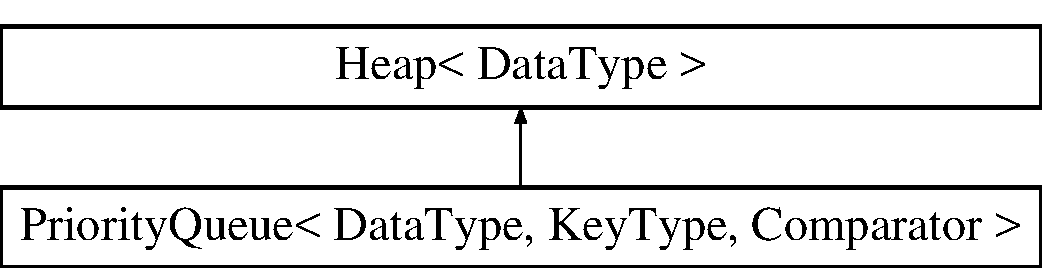
\includegraphics[height=2.000000cm]{class_priority_queue}
\end{center}
\end{figure}
\subsubsection*{Public Member Functions}
\begin{DoxyCompactItemize}
\item 
\hyperlink{class_priority_queue_a47de2a46cff1d6a6ed30a99c94dc1b14}{Priority\+Queue} (int max\+Number=def\+Max\+Queue\+Size)
\item 
void \hyperlink{class_priority_queue_a61f3339cf0e87c67ed004f8eff0a1bfa}{enqueue} (const Data\+Type \&new\+Data\+Item)
\item 
Data\+Type \hyperlink{class_priority_queue_a5bc758e313d6244e672ea6e81d695a46}{dequeue} ()
\end{DoxyCompactItemize}
\subsubsection*{Additional Inherited Members}


\subsubsection{Constructor \& Destructor Documentation}
\index{Priority\+Queue@{Priority\+Queue}!Priority\+Queue@{Priority\+Queue}}
\index{Priority\+Queue@{Priority\+Queue}!Priority\+Queue@{Priority\+Queue}}
\paragraph[{\texorpdfstring{Priority\+Queue(int max\+Number=def\+Max\+Queue\+Size)}{PriorityQueue(int maxNumber=defMaxQueueSize)}}]{\setlength{\rightskip}{0pt plus 5cm}template$<$typename Data\+Type , typename Key\+Type , typename Comparator $>$ {\bf Priority\+Queue}$<$ Data\+Type, Key\+Type, Comparator $>$\+::{\bf Priority\+Queue} (
\begin{DoxyParamCaption}
\item[{int}]{max\+Number = {\ttfamily defMaxQueueSize}}
\end{DoxyParamCaption}
)}\hypertarget{class_priority_queue_a47de2a46cff1d6a6ed30a99c94dc1b14}{}\label{class_priority_queue_a47de2a46cff1d6a6ed30a99c94dc1b14}
This function is the constructor for the \hyperlink{class_priority_queue}{Priority\+Queue} class.

This function calls the base class implementation of the heap constructor, with the pass parameter max\+Number as the parameter.


\begin{DoxyParams}{Parameters}
{\em int} & max\+Number, which is the largest possible size for the priorityqueue \\
\hline
\end{DoxyParams}
\begin{DoxyReturn}{Returns}
This function does not return anything.
\end{DoxyReturn}
\begin{DoxyPrecond}{Precondition}
none 
\end{DoxyPrecond}
\begin{DoxyPostcond}{Postcondition}
The priotity queue is empty and has been dynamically allocated to have the max\+Number equal to the size. 
\end{DoxyPostcond}


\subsubsection{Member Function Documentation}
\index{Priority\+Queue@{Priority\+Queue}!dequeue@{dequeue}}
\index{dequeue@{dequeue}!Priority\+Queue@{Priority\+Queue}}
\paragraph[{\texorpdfstring{dequeue()}{dequeue()}}]{\setlength{\rightskip}{0pt plus 5cm}template$<$typename Data\+Type , typename Key\+Type , typename Comparator $>$ Data\+Type {\bf Priority\+Queue}$<$ Data\+Type, Key\+Type, Comparator $>$\+::dequeue (
\begin{DoxyParamCaption}
{}
\end{DoxyParamCaption}
)}\hypertarget{class_priority_queue_a5bc758e313d6244e672ea6e81d695a46}{}\label{class_priority_queue_a5bc758e313d6244e672ea6e81d695a46}
This function is the dequeue function for the \hyperlink{class_priority_queue}{Priority\+Queue} class.

This function calls the base class implementation of the remove function and returns return of the remove function.


\begin{DoxyParams}{Parameters}
{\em none} & \\
\hline
\end{DoxyParams}
\begin{DoxyReturn}{Returns}
This function returns true or false depending on if the item was dequeued.
\end{DoxyReturn}
\begin{DoxyPrecond}{Precondition}
none 
\end{DoxyPrecond}
\begin{DoxyPostcond}{Postcondition}
This function dequeues the top item of the priorityqueue and returns true or false depending on if the item was dequeued. 
\end{DoxyPostcond}
\index{Priority\+Queue@{Priority\+Queue}!enqueue@{enqueue}}
\index{enqueue@{enqueue}!Priority\+Queue@{Priority\+Queue}}
\paragraph[{\texorpdfstring{enqueue(const Data\+Type \&new\+Data\+Item)}{enqueue(const DataType &newDataItem)}}]{\setlength{\rightskip}{0pt plus 5cm}template$<$typename Data\+Type , typename Key\+Type , typename Comparator $>$ void {\bf Priority\+Queue}$<$ Data\+Type, Key\+Type, Comparator $>$\+::enqueue (
\begin{DoxyParamCaption}
\item[{const Data\+Type \&}]{newdata\+Item}
\end{DoxyParamCaption}
)}\hypertarget{class_priority_queue_a61f3339cf0e87c67ed004f8eff0a1bfa}{}\label{class_priority_queue_a61f3339cf0e87c67ed004f8eff0a1bfa}
This function is the insert function for the \hyperlink{class_priority_queue}{Priority\+Queue} class.

This function calls the base class implementation of the insert function, with the passed parameter newdata\+Item as the parameter.


\begin{DoxyParams}{Parameters}
{\em const} & Data\+Type \&new\+Data\+Item, the data\+Item to be inserted. \\
\hline
\end{DoxyParams}
\begin{DoxyReturn}{Returns}
This function does not return anything.
\end{DoxyReturn}
\begin{DoxyPrecond}{Precondition}
none 
\end{DoxyPrecond}
\begin{DoxyPostcond}{Postcondition}
Inserts a new item into the priority\+Queue. 
\end{DoxyPostcond}


The documentation for this class was generated from the following files\+:\begin{DoxyCompactItemize}
\item 
Priority\+Queue.\+h\item 
\hyperlink{_priority_queue_8cpp}{Priority\+Queue.\+cpp}\end{DoxyCompactItemize}

\hypertarget{struct_task_data}{}\subsection{Task\+Data Struct Reference}
\label{struct_task_data}\index{Task\+Data@{Task\+Data}}
\subsubsection*{Public Member Functions}
\begin{DoxyCompactItemize}
\item 
int {\bfseries get\+Priority} () const \hypertarget{struct_task_data_a58cbe6eec8a86be7b827561a2f4b49c1}{}\label{struct_task_data_a58cbe6eec8a86be7b827561a2f4b49c1}

\end{DoxyCompactItemize}
\subsubsection*{Public Attributes}
\begin{DoxyCompactItemize}
\item 
int {\bfseries priority}\hypertarget{struct_task_data_a9d8b606897eb428a62d816b71312e1b7}{}\label{struct_task_data_a9d8b606897eb428a62d816b71312e1b7}

\item 
int {\bfseries arrived}\hypertarget{struct_task_data_a126fafee3369b6a2d8734f4e46c670bc}{}\label{struct_task_data_a126fafee3369b6a2d8734f4e46c670bc}

\end{DoxyCompactItemize}


The documentation for this struct was generated from the following file\+:\begin{DoxyCompactItemize}
\item 
ossim.\+cpp\end{DoxyCompactItemize}

\hypertarget{class_test_data}{}\subsection{Test\+Data Class Reference}
\label{class_test_data}\index{Test\+Data@{Test\+Data}}
\subsubsection*{Public Member Functions}
\begin{DoxyCompactItemize}
\item 
\hyperlink{class_test_data_aa4a3dd519ba3a3ae02956b627d42d123}{Test\+Data} ()
\item 
void \hyperlink{class_test_data_a72cb0d5febcf77e8a6dd494fa6dff411}{set\+Key} (const string \&new\+Key)
\item 
string \hyperlink{class_test_data_ae20d0a4c5fba891d728c68ac4ec79654}{get\+Key} () const 
\item 
void \hyperlink{class_test_data_ac7fe71dc8c3eda2242e443d22523e286}{set\+Value} (const string \&new\+Value)
\item 
string \hyperlink{class_test_data_af33e667b6962f8a351f7a660a1a24c5e}{get\+Value} () const 
\item 
void {\bfseries set\+Key} (const string \&new\+Key)\hypertarget{class_test_data_a72cb0d5febcf77e8a6dd494fa6dff411}{}\label{class_test_data_a72cb0d5febcf77e8a6dd494fa6dff411}

\item 
string {\bfseries get\+Key} () const \hypertarget{class_test_data_ae20d0a4c5fba891d728c68ac4ec79654}{}\label{class_test_data_ae20d0a4c5fba891d728c68ac4ec79654}

\item 
int {\bfseries get\+Value} () const \hypertarget{class_test_data_af33e667b6962f8a351f7a660a1a24c5e}{}\label{class_test_data_af33e667b6962f8a351f7a660a1a24c5e}

\end{DoxyCompactItemize}
\subsubsection*{Static Public Member Functions}
\begin{DoxyCompactItemize}
\item 
static unsigned int {\bfseries hash} (const string \&str)\hypertarget{class_test_data_a55f0e2851aa330be9921303107982f98}{}\label{class_test_data_a55f0e2851aa330be9921303107982f98}

\item 
static unsigned int {\bfseries hash} (const string \&str)\hypertarget{class_test_data_ac38bf2161ad472cfa80703a87e7eda8a}{}\label{class_test_data_ac38bf2161ad472cfa80703a87e7eda8a}

\end{DoxyCompactItemize}
\subsubsection*{Private Attributes}
\begin{DoxyCompactItemize}
\item 
string {\bfseries key}\hypertarget{class_test_data_a16fe3a9a89c54e55fc56ae88590ae0c8}{}\label{class_test_data_a16fe3a9a89c54e55fc56ae88590ae0c8}

\item 
string {\bfseries value}\hypertarget{class_test_data_a7ac7d757d4e86c21d6263bd3ad03cdd3}{}\label{class_test_data_a7ac7d757d4e86c21d6263bd3ad03cdd3}

\item 
int {\bfseries value}\hypertarget{class_test_data_a8291f6b900b25a926deb1b2a393dc0ff}{}\label{class_test_data_a8291f6b900b25a926deb1b2a393dc0ff}

\end{DoxyCompactItemize}
\subsubsection*{Static Private Attributes}
\begin{DoxyCompactItemize}
\item 
static int {\bfseries count} = 0\hypertarget{class_test_data_a9209c5345dda5dcb483b9c972fafc495}{}\label{class_test_data_a9209c5345dda5dcb483b9c972fafc495}

\end{DoxyCompactItemize}


\subsubsection{Constructor \& Destructor Documentation}
\index{Test\+Data@{Test\+Data}!Test\+Data@{Test\+Data}}
\index{Test\+Data@{Test\+Data}!Test\+Data@{Test\+Data}}
\paragraph[{\texorpdfstring{Test\+Data()}{TestData()}}]{\setlength{\rightskip}{0pt plus 5cm}Test\+Data\+::\+Test\+Data (
\begin{DoxyParamCaption}
{}
\end{DoxyParamCaption}
)}\hypertarget{class_test_data_aa4a3dd519ba3a3ae02956b627d42d123}{}\label{class_test_data_aa4a3dd519ba3a3ae02956b627d42d123}
This function is the constructor for the \hyperlink{class_test_data}{Test\+Data} class.

This function does nothing.


\begin{DoxyParams}{Parameters}
{\em none} & \\
\hline
\end{DoxyParams}
\begin{DoxyReturn}{Returns}
This function does not return anything.
\end{DoxyReturn}
\begin{DoxyPrecond}{Precondition}
nothing. 
\end{DoxyPrecond}
\begin{DoxyPostcond}{Postcondition}
nothing. 
\end{DoxyPostcond}


\subsubsection{Member Function Documentation}
\index{Test\+Data@{Test\+Data}!get\+Key@{get\+Key}}
\index{get\+Key@{get\+Key}!Test\+Data@{Test\+Data}}
\paragraph[{\texorpdfstring{get\+Key() const }{getKey() const }}]{\setlength{\rightskip}{0pt plus 5cm}string Test\+Data\+::get\+Key (
\begin{DoxyParamCaption}
{}
\end{DoxyParamCaption}
) const}\hypertarget{class_test_data_ae20d0a4c5fba891d728c68ac4ec79654}{}\label{class_test_data_ae20d0a4c5fba891d728c68ac4ec79654}
This function is the get\+Key for the \hyperlink{class_test_data}{Test\+Data} class.

This function returns the key(user) string.


\begin{DoxyParams}{Parameters}
{\em none} & \\
\hline
\end{DoxyParams}
\begin{DoxyReturn}{Returns}
This function returns the key(user) string.
\end{DoxyReturn}
\begin{DoxyPrecond}{Precondition}
nothing. 
\end{DoxyPrecond}
\begin{DoxyPostcond}{Postcondition}
This function returns the key(user) string. 
\end{DoxyPostcond}
\index{Test\+Data@{Test\+Data}!get\+Value@{get\+Value}}
\index{get\+Value@{get\+Value}!Test\+Data@{Test\+Data}}
\paragraph[{\texorpdfstring{get\+Value() const }{getValue() const }}]{\setlength{\rightskip}{0pt plus 5cm}int Test\+Data\+::get\+Value (
\begin{DoxyParamCaption}
{}
\end{DoxyParamCaption}
) const}\hypertarget{class_test_data_af33e667b6962f8a351f7a660a1a24c5e}{}\label{class_test_data_af33e667b6962f8a351f7a660a1a24c5e}
This function is the get\+Value function for the \hyperlink{class_test_data}{Test\+Data} class.

This function returns the Value(password) string.


\begin{DoxyParams}{Parameters}
{\em none} & \\
\hline
\end{DoxyParams}
\begin{DoxyReturn}{Returns}
This function returns the Value(password) string.
\end{DoxyReturn}
\begin{DoxyPrecond}{Precondition}
nothing. 
\end{DoxyPrecond}
\begin{DoxyPostcond}{Postcondition}
This function returns the Value(password) string. 
\end{DoxyPostcond}
\index{Test\+Data@{Test\+Data}!set\+Key@{set\+Key}}
\index{set\+Key@{set\+Key}!Test\+Data@{Test\+Data}}
\paragraph[{\texorpdfstring{set\+Key(const string \&new\+Key)}{setKey(const string &newKey)}}]{\setlength{\rightskip}{0pt plus 5cm}void Test\+Data\+::set\+Key (
\begin{DoxyParamCaption}
\item[{const string \&}]{new\+Key}
\end{DoxyParamCaption}
)}\hypertarget{class_test_data_a72cb0d5febcf77e8a6dd494fa6dff411}{}\label{class_test_data_a72cb0d5febcf77e8a6dd494fa6dff411}
This function is the set\+Key function for the \hyperlink{class_test_data}{Test\+Data} class.

This function will set the string key equal to new\+Key.


\begin{DoxyParams}{Parameters}
{\em const} & string\& new\+Key, which is the string to be user of the class. \\
\hline
\end{DoxyParams}
\begin{DoxyReturn}{Returns}
This function does not return anything.
\end{DoxyReturn}
\begin{DoxyPrecond}{Precondition}
A \hyperlink{class_test_data}{Test\+Data} class. 
\end{DoxyPrecond}
\begin{DoxyPostcond}{Postcondition}
Key will now be equal to new\+Key. 
\end{DoxyPostcond}
\index{Test\+Data@{Test\+Data}!set\+Value@{set\+Value}}
\index{set\+Value@{set\+Value}!Test\+Data@{Test\+Data}}
\paragraph[{\texorpdfstring{set\+Value(const string \&new\+Value)}{setValue(const string &newValue)}}]{\setlength{\rightskip}{0pt plus 5cm}void Test\+Data\+::set\+Value (
\begin{DoxyParamCaption}
\item[{const string \&}]{new\+Value}
\end{DoxyParamCaption}
)}\hypertarget{class_test_data_ac7fe71dc8c3eda2242e443d22523e286}{}\label{class_test_data_ac7fe71dc8c3eda2242e443d22523e286}
This function is the set\+Value function for the \hyperlink{class_test_data}{Test\+Data} class.

This function will set the string value equal to new\+Value.


\begin{DoxyParams}{Parameters}
{\em const} & string\& new\+Value, which is the string to be password of the class. \\
\hline
\end{DoxyParams}
\begin{DoxyReturn}{Returns}
This function does not return anything.
\end{DoxyReturn}
\begin{DoxyPrecond}{Precondition}
A \hyperlink{class_test_data}{Test\+Data} class. 
\end{DoxyPrecond}
\begin{DoxyPostcond}{Postcondition}
Value will now be equal to new\+Value. 
\end{DoxyPostcond}


The documentation for this class was generated from the following files\+:\begin{DoxyCompactItemize}
\item 
\hyperlink{login_8cpp}{login.\+cpp}\item 
test10.\+cpp\end{DoxyCompactItemize}

\hypertarget{class_test_data_item}{}\subsection{Test\+Data\+Item$<$ Key\+Type $>$ Class Template Reference}
\label{class_test_data_item}\index{Test\+Data\+Item$<$ Key\+Type $>$@{Test\+Data\+Item$<$ Key\+Type $>$}}
\subsubsection*{Public Member Functions}
\begin{DoxyCompactItemize}
\item 
void {\bfseries set\+Priority} (Key\+Type new\+Pty)\hypertarget{class_test_data_item_a84667429c081b1dbb212956c88011216}{}\label{class_test_data_item_a84667429c081b1dbb212956c88011216}

\item 
Key\+Type {\bfseries get\+Priority} () const \hypertarget{class_test_data_item_ac1632213d959555ec8f5aee8a1505d72}{}\label{class_test_data_item_ac1632213d959555ec8f5aee8a1505d72}

\end{DoxyCompactItemize}
\subsubsection*{Private Attributes}
\begin{DoxyCompactItemize}
\item 
Key\+Type {\bfseries priority}\hypertarget{class_test_data_item_a9b1a2617cb7a831206d189559e8e2e8b}{}\label{class_test_data_item_a9b1a2617cb7a831206d189559e8e2e8b}

\end{DoxyCompactItemize}


The documentation for this class was generated from the following file\+:\begin{DoxyCompactItemize}
\item 
test11.\+cpp\end{DoxyCompactItemize}

\section{File Documentation}
\hypertarget{_heap_8cpp}{}\subsection{Heap.\+cpp File Reference}
\label{_heap_8cpp}\index{Heap.\+cpp@{Heap.\+cpp}}


This program will implement a Hash\+Table using a Binary Search Tree A\+DT.  


{\ttfamily \#include \char`\"{}Heap.\+h\char`\"{}}\\*


\subsubsection{Detailed Description}
This program will implement a Hash\+Table using a Binary Search Tree A\+DT. 

\begin{DoxyAuthor}{Author}
Kripash Shrestha 
\end{DoxyAuthor}
\begin{DoxyVersion}{Version}
1.\+0
\end{DoxyVersion}
The specifications of the program are instructed and documented on Lab 11 C++ Data Structures\+: A Laboratory Course Third Edition by Brandle, Geisler, Roberge and Whittington \begin{DoxyDate}{Date}
Wednesday, November 15, 2017 
\end{DoxyDate}

\hypertarget{_priority_queue_8cpp}{}\subsection{Priority\+Queue.\+cpp File Reference}
\label{_priority_queue_8cpp}\index{Priority\+Queue.\+cpp@{Priority\+Queue.\+cpp}}


This program will implement a inheritance class called Priority queue to develop a simulation of an operating system\textquotesingle{}s task schedule using a priority queue.  


{\ttfamily \#include \char`\"{}Priority\+Queue.\+h\char`\"{}}\\*


\subsubsection{Detailed Description}
This program will implement a inheritance class called Priority queue to develop a simulation of an operating system\textquotesingle{}s task schedule using a priority queue. 

\begin{DoxyAuthor}{Author}
Kripash Shrestha 
\end{DoxyAuthor}
\begin{DoxyVersion}{Version}
1.\+0
\end{DoxyVersion}
The specifications of the program are instructed and documented on Lab 11 C++ Data Structures\+: A Laboratory Course Third Edition by Brandle, Geisler, Roberge and Whittington \begin{DoxyDate}{Date}
Wednesday, November 15, 2017 
\end{DoxyDate}

%--- End generated contents ---

% Index
\newpage
\phantomsection
\clearemptydoublepage
\addcontentsline{toc}{section}{Index}
\printindex

\end{document}
